\subsection{Dam-break problem}%ETSIN experimental tests

The objectives of this section are to compare experimental measurements on dam-break flow over a dry horizontal bed with the numerical approximation carried out with the pfem algorithm. The extensive set of experimental data is extracted from \cite{Lobovsky13}, where the dynamics of the dam break wave impacting a vertical wall downstream the dam, with emphasis on the pressure loads and surface evolution after the dam burst, are presented.

Computational configuration of the tank used in experimental cases is presented in Figure \ref{fg:dambreak-config}. There, the locations of water level measuring points and pressure sensors are shown. In this report only the case with $H=300[mm]$ is analyzed. Two-phase non-viscous flow simulation is carried on, with $\rho_{water}=1000[kg/m^3]$ and $\rho_{air}=1[kg/m^3]$ with a gravity force $\mathbf{g}=-10\ \hat{j} [m/s^2]$. The 2D computational grid used has $322\times120$ nodes, conforming a mesh with around $80000$ triangles. Boundary conditions are slip on all walls, and $\Delta t$ is fixed to $0.1$, which allows to reach $CFL_{max}\approx20$ when free surface impacts the downstream wall.

\begin{figure}[htbp]
  \begin{center}
      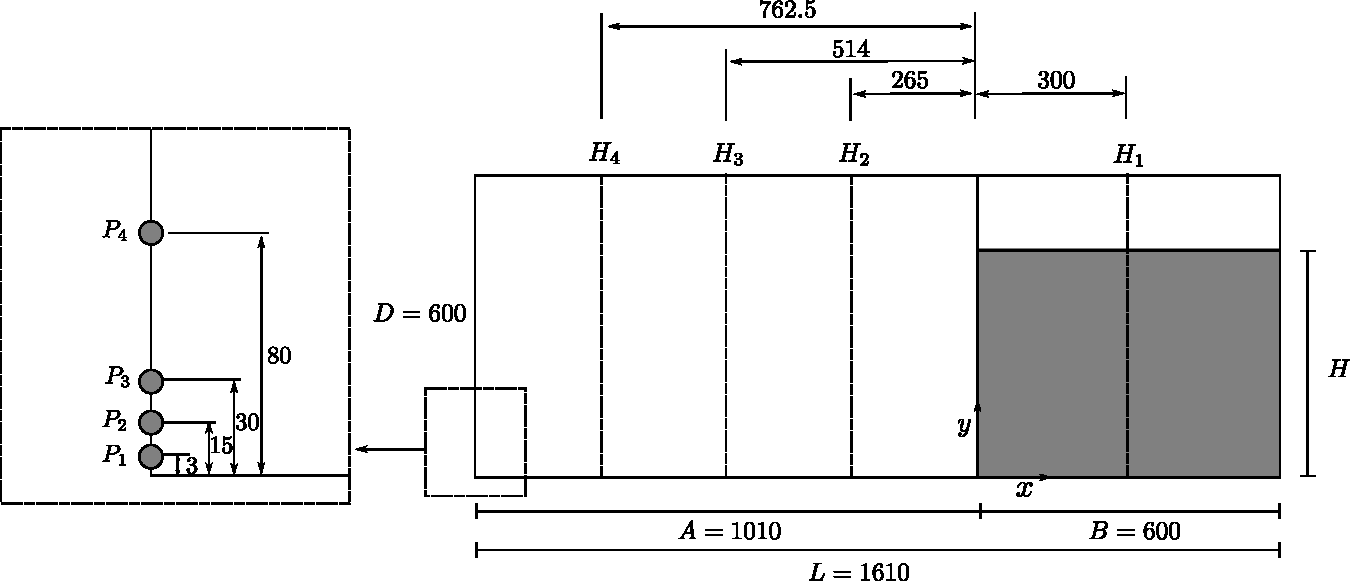
\includegraphics[width=\columnwidth]{images/dam_break_config.pdf}
  \end{center}
  \caption{\label{fg:dambreak-config} Configuration scheme of the dam-break case. $H_1$, $H_2$, $H_3$, $H_4$ present the locations of water level measuring positions. Also, $P_1$, $P_2$, $P_3$, $P_4$ show the locations of pressure sensors at the impact wall downstream the dam. Grey zone represents the initial condition. Dimensions in millimeters.}
\end{figure}

Figure \ref{fg:dambreak-h} shows the comparison between experimental and numerical results for each water-level measurement. A good agreement can be observed, moreover taken into account the capture of the back wave and splashing start events.
  \begin{figure}[h]
  \centering
    \subfloat[]{
	  \label{fg:dambreak-h1}         %% Etiqueta para la primera subfigura
	  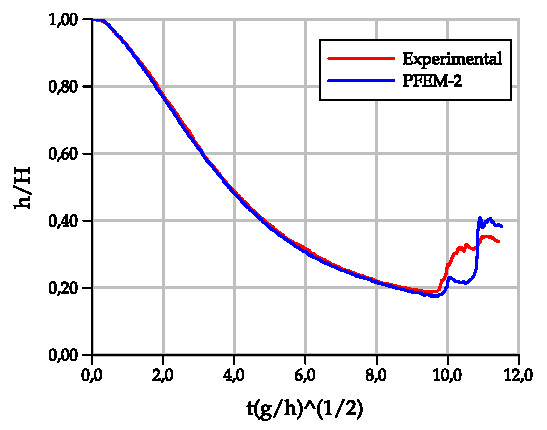
\includegraphics[width=.48\columnwidth]{images/dambreak_h1.pdf}
    }
    %%----segunda subfigura----
    \subfloat[]{
	  \label{fg:dambreak-h2}         %% Etiqueta para la segunda subfigura
	  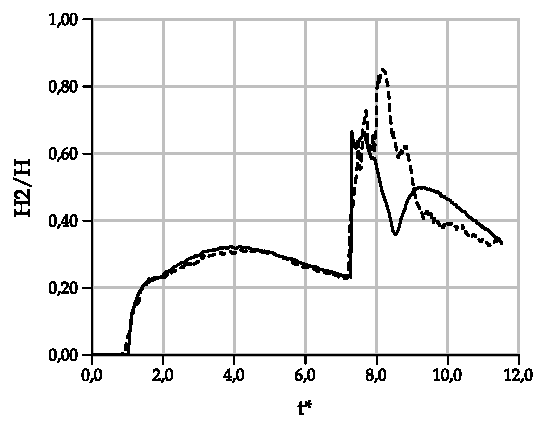
\includegraphics[width=.48\columnwidth]{images/dambreak_h2.pdf}
    } \\
    \subfloat[]{
	  \label{fg:dambreak-h3}         %% Etiqueta para la primera subfigura
	  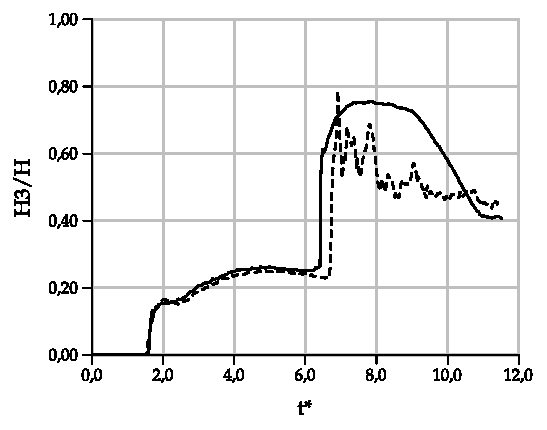
\includegraphics[width=.48\columnwidth]{images/dambreak_h3.pdf}
    }
    %%----segunda subfigura----
    \subfloat[]{
	  \label{fg:dambreak-h4}         %% Etiqueta para la segunda subfigura
	  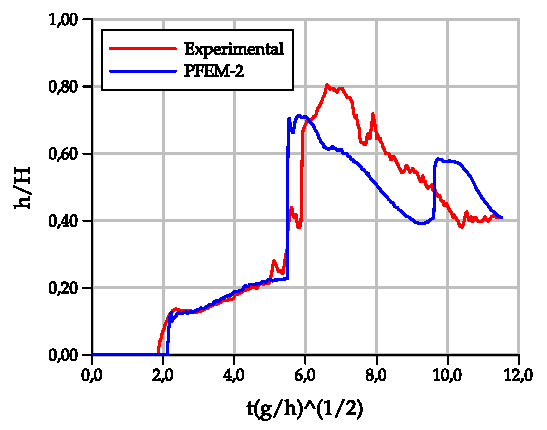
\includegraphics[width=.48\columnwidth]{images/dambreak_h4.pdf}
    }
   \caption{Water level elevations at locations $H_1$, $H_2$, $H_3$ and $H_4$ for tests with $H=300[mm]$ initial filling height compared to data from literature experimental results\cite{Lobovsky13} and numerical results with PFEM-2.}
   \label{fg:dambreak-h}                %% Etiqueta para la figura entera
\end{figure}

The impact pressure was measured with four sensors at the vertical wall at the end of the downstream flume, as described in Figure \ref{fg:dambreak-config}. The statistical analysis of the pressure peaks, rise times and the occurrence time, i.e. the time between
the opening of the dam gate and the occurrence of the impact, is presented in Figure \ref{fg:dambreak-p}. The shown pressure $P$ is non-dimensionalized with regards to the hydrostatic pressure at the bottom of the reservoir and denoted as $P^∗$.

In the reference work, the analysis is focused on peaks events. It can be noticed that the highest peak is recorded by sensor number 1 which is the sensor receiving the full impact, whilst the pressure of the other sensors is given by the run up of the flow. It can also be observed that sensor number 4, i.e. the sensor located at the highest position, does not show a pure impact event, see Figure \ref{fg:dambreak-p4}, and actually the maximum for this sensor is obtained later in time, when the water falls back after running along the wall. Numerical solution behavior follows the mentioned conclusions, but the pressure values are not between the statistical limits of experimental data. Also, a discrepancy can be observed with the peaks times for sensors $1$ to $3$. This difference can be assigned to the numerical simplification which does not model the gate movement.

  \begin{figure}[h]
  \centering
    \subfloat[]{
	  \label{fg:dambreak-p1}         %% Etiqueta para la primera subfigura
	  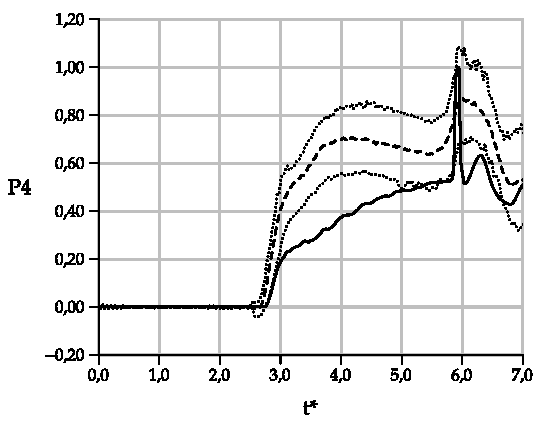
\includegraphics[width=.48\columnwidth]{images/dambreak_p4.pdf}
    }
    %%----segunda subfigura----
    \subfloat[]{
	  \label{fg:dambreak-p2}         %% Etiqueta para la segunda subfigura
	  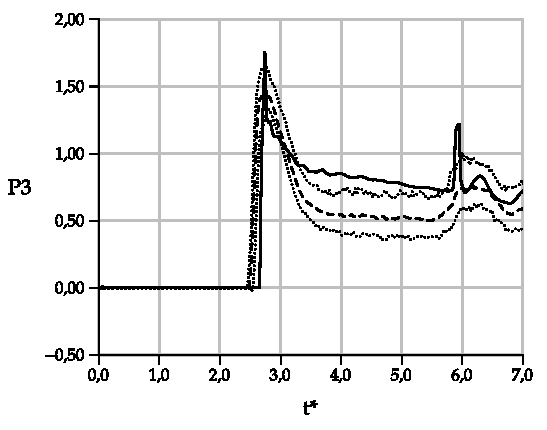
\includegraphics[width=.48\columnwidth]{images/dambreak_p3.pdf}
    } \\
    \subfloat[]{
	  \label{fg:dambreak-p3}         %% Etiqueta para la primera subfigura
	  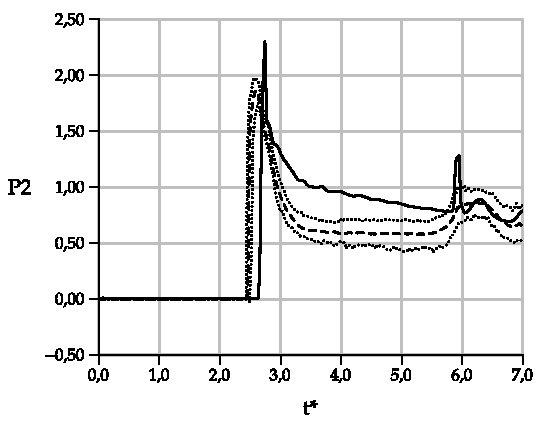
\includegraphics[width=.48\columnwidth]{images/dambreak_p2.pdf}
    }
    %%----segunda subfigura----
    \subfloat[]{
	  \label{fg:dambreak-p4}         %% Etiqueta para la segunda subfigura
	  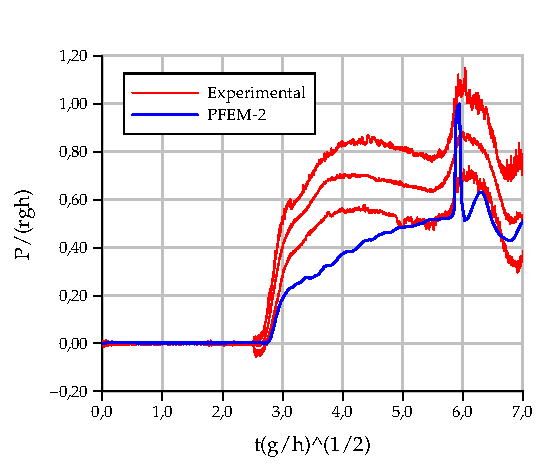
\includegraphics[width=.48\columnwidth]{images/dambreak_p1.pdf}
    }
   \caption{Pressure time histories comparison between experimental results\cite{Lobovsky13} and numerical results with PFEM-2. Locations $P_1$, $P_2$, $P_3$, $P_4$ area presented in Figures \ref{fg:dambreak-p1},\ref{fg:dambreak-p2},\ref{fg:dambreak-p3},\ref{fg:dambreak-p4} respectively. Experimental results shows the median and percentiles $2.5$ and $97.5$.}
   \label{fg:dambreak-p}                %% Etiqueta para la figura entera
\end{figure}

  \begin{figure}[H]
  \centering
    \subfloat[]{
	  \label{fg:dambreak-1}
	  
\includegraphics[width=.48\columnwidth]{images/dambreak_pfem_1.jpg}
    }
    %%----segunda subfigura----
    \subfloat[]{
	  \label{fg:dambreak-2}
	  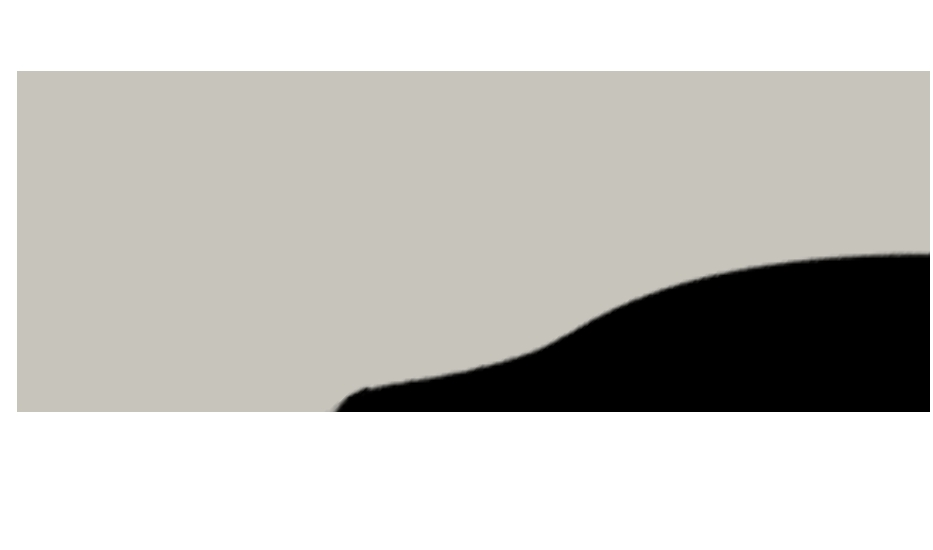
\includegraphics[width=.48\columnwidth]{images/dambreak_pfem_2.jpg}
    } \\
    \subfloat[]{
	  \label{fg:dambreak-3}
	  
\includegraphics[width=.48\columnwidth]{images/dambreak_pfem_3.jpg}
    }
    %%----segunda subfigura----
    \subfloat[]{
	  \label{fg:dambreak-4}
	  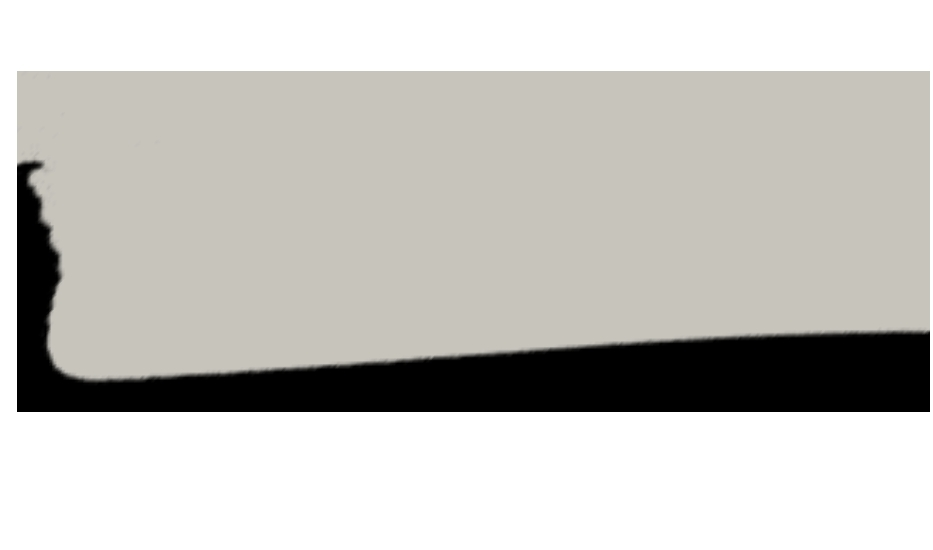
\includegraphics[width=.48\columnwidth]{images/dambreak_pfem_4.jpg}
    }\\
        \subfloat[]{
	  \label{fg:dambreak-5}
	  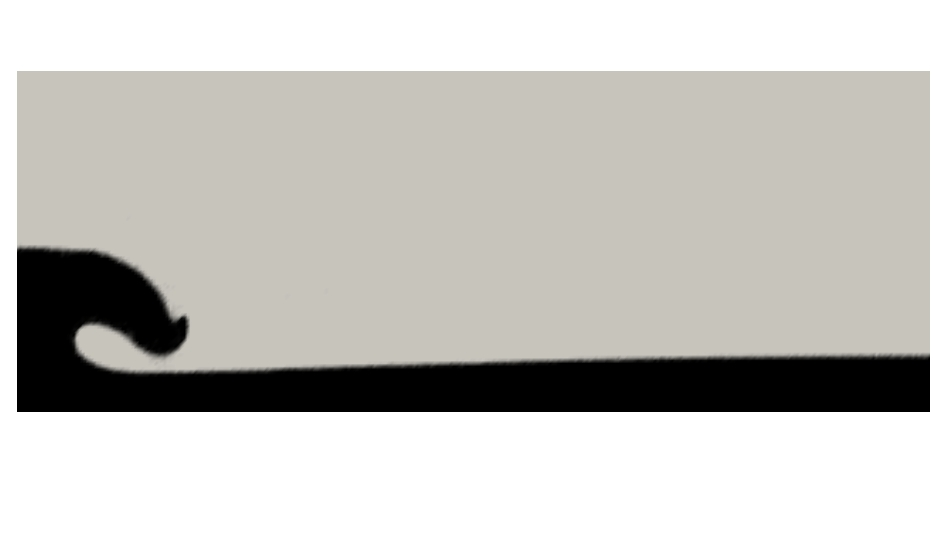
\includegraphics[width=.48\columnwidth]{images/dambreak_pfem_5.jpg}
    }
    %%----segunda subfigura----
    \subfloat[]{
	  \label{fg:dambreak-6}
	  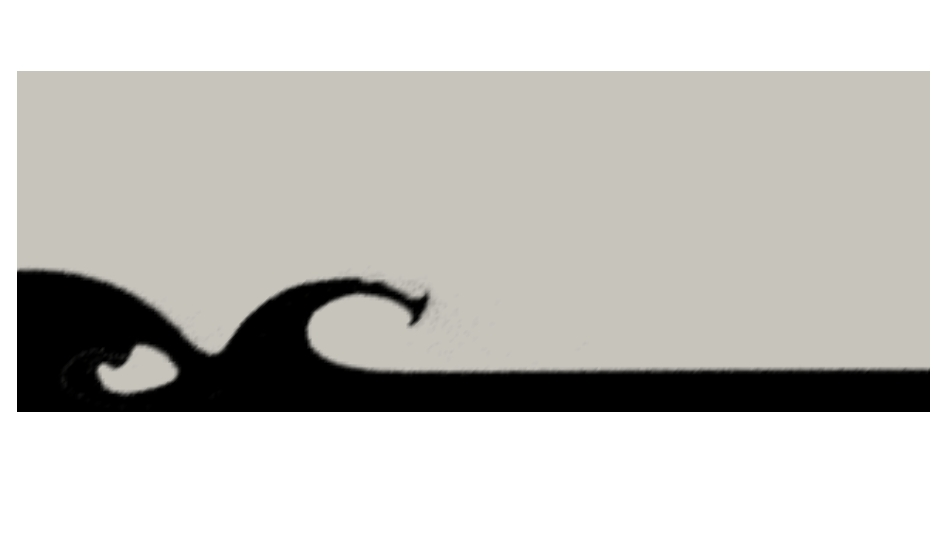
\includegraphics[width=.48\columnwidth]{images/dambreak_pfem_6.jpg}
    } \\
    \subfloat[]{
	  \label{fg:dambreak-7}
	  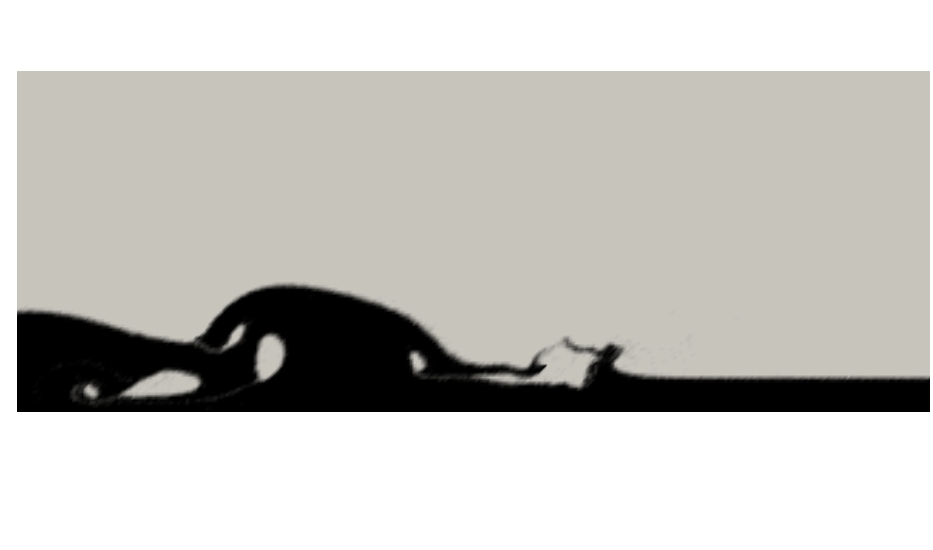
\includegraphics[width=.48\columnwidth]{images/dambreak_pfem_7.jpg}
    }
    %%----segunda subfigura----
    \subfloat[]{
	  \label{fg:dambreak-8}
	  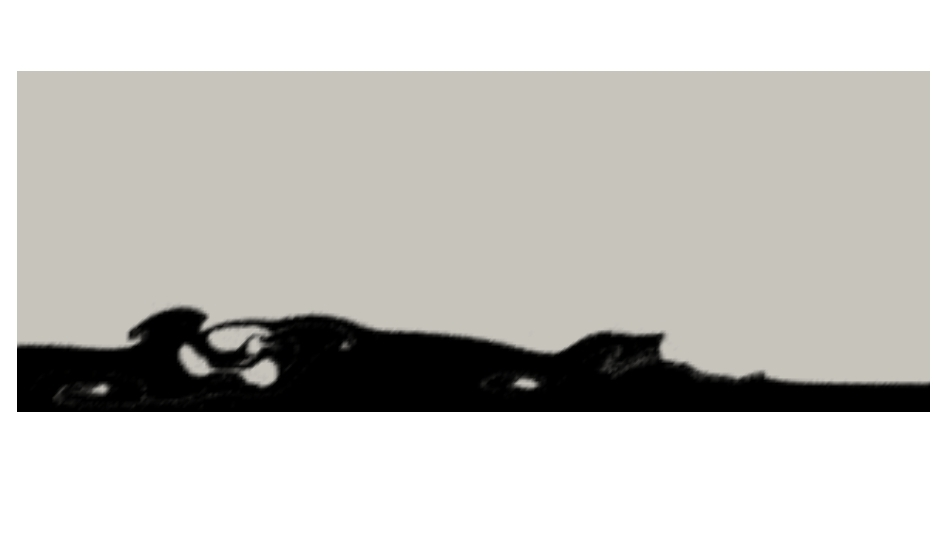
\includegraphics[width=.48\columnwidth]{images/dambreak_pfem_8.jpg}
    }
   \caption{Snapshots of the dam-break at times $t=0,0.25,0.5,0.75,1,1.25,1.5,1.75[s]$.}
   \label{fg:dambreak-screenshots}
\end{figure}
\clearpage
